%----------------------------------------------------------------------------------------
\begin{frame}
 \frametitle{TGV {\small Taylor-Green Vortex flow}}
 \textbf{Monolithc vs Segregated Runge-Kutta:}
 \vspace*{-0.3cm}
   \begin{figure}
     \centering	
     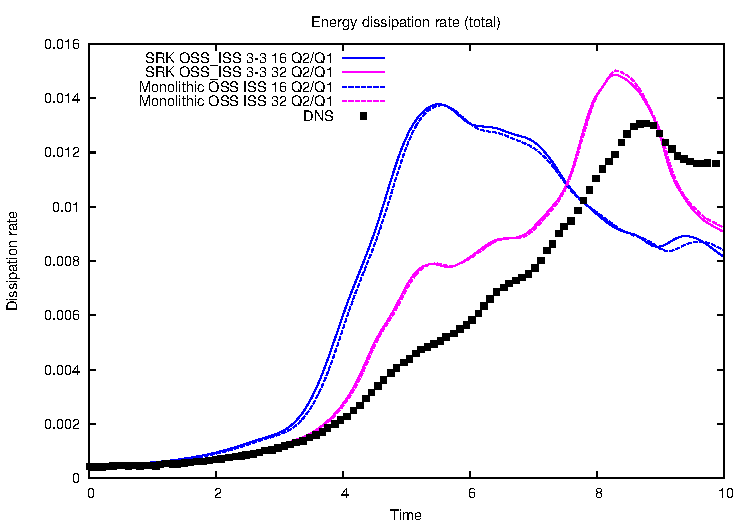
\includegraphics[width=0.65\textwidth]{Figures/plt_tg3d_tot.pdf}
     \vspace*{-0.3cm}
     \caption{Total energy dissipation rate}
   \end{figure}
 \begin{overlayarea}{\textwidth}{1.5cm}
 \only<2->{
 \vspace*{-0.5cm}
 \begin{itemize}
   	\item Almost \alert<2>{Identical results} obtained with Crank-Nicolson
   	\only<3->{\item \alert<3>{Velocity-pressure segregation and adaptive} time stepping}
  \end{itemize}}
  \end{overlayarea}
\end{frame}
%----------------------------------------------------------------------------------------
\begin{frame}
 \frametitle{TGV {\small Taylor-Green Vortex flow}}
 \textbf{Weak scalability:} HLRN-III Cray XC40 with Intel Xeon Haswell
 \vspace*{-0.1cm}
   \only<1-3>{
   \begin{figure}
     \centering	
     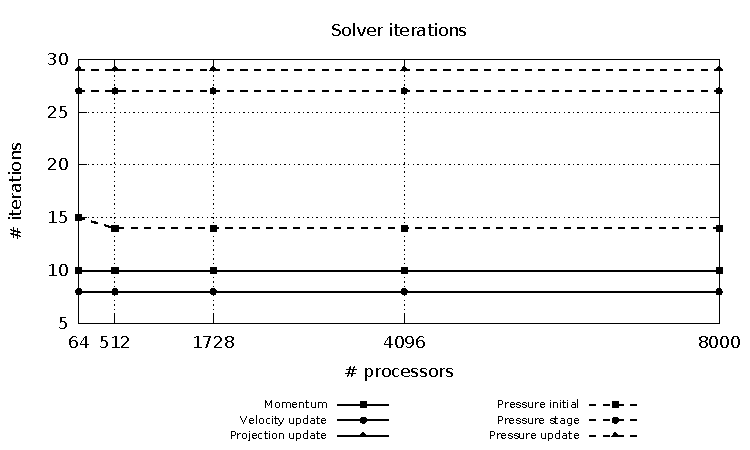
\includegraphics[width=0.75\textwidth]{Figures/iter_12_ce.pdf}
     \vspace*{-0.3cm}
     \caption{Solver iterations}
   \end{figure}}
   \only<4->{
   \begin{figure}
     \centering	
     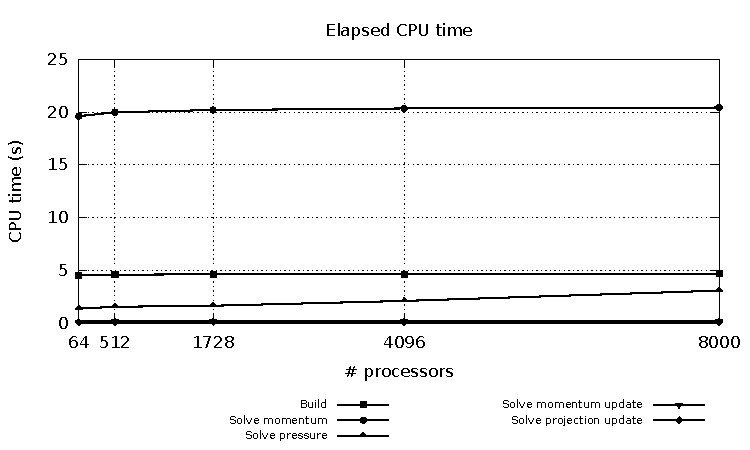
\includegraphics[width=0.75\textwidth]{Figures/time_12_ce.pdf}
     \vspace*{-0.3cm}
     \caption{CPU time}
   \end{figure}}
 \begin{overlayarea}{\textwidth}{1.5cm}
 \vspace*{-0.5cm}
 \only<2-3>{
 \begin{itemize}
   	\item \alert<2>{Perfect scalability} in terms of solver iterations
   	\only<3->{\item \alert<3>{Darcy-type} problem requires \alert<3>{more iterations}}
  \end{itemize}}
 \only<5->{
 \begin{itemize}
   	\item \alert<5>{Perfect scalability} in CPU time consumed
   	\only<6->{\item \alert<6>{Momentum} problem requires \alert<6>{more time}}
  \end{itemize}}
  \end{overlayarea}
\end{frame}